% \iffalse
\let\negmedspace\undefined
\let\negthickspace\undefined
\documentclass[journal,12pt,twocolumn]{IEEEtran}
\usepackage{cite}
\usepackage{amsmath,amssymb,amsfonts,amsthm}
\usepackage{algorithmic}
\usepackage{graphicx}
\usepackage{textcomp}
\usepackage{xcolor}
\usepackage{txfonts}
\usepackage{listings}
\usepackage{enumitem}
\usepackage{mathtools}
\usepackage{gensymb}
\usepackage{comment}
\usepackage[breaklinks=true]{hyperref}
\usepackage{tkz-euclide}
\usepackage{listings}
\usepackage{gvv}
\def\inputGnumericTable{}
\usepackage[latin1]{inputenc}
\usepackage{color}
\usepackage{array}
\usepackage{longtable}
\usepackage{calc}
\usepackage{multirow}
\usepackage{hhline}
\usepackage{ifthen}
\usepackage{lscape}

\newtheorem{theorem}{Theorem}[section]
\newtheorem{problem}{Problem}
\newtheorem{proposition}{Proposition}[section]
\newtheorem{lemma}{Lemma}[section]
\newtheorem{corollary}[theorem]{Corollary}
\newtheorem{example}{Example}[section]
\newtheorem{definition}[problem]{Definition}
\newcommand{\BEQA}{\begin{eqnarray}}
\newcommand{\EEQA}{\end{eqnarray}}
\newcommand{\define}{\stackrel{\triangle}{=}}
\theoremstyle{remark}
\newtheorem{rem}{Remark}
\begin{document}

\bibliographystyle{IEEEtran}
\vspace{3cm}

\title{NCERT Discrete - 11.9.3.30}
\author{EE23BTECH11007 - Aneesh Kadiyala$^{*}$% <-this % stops a space
}
\maketitle
\newpage
\bigskip

\renewcommand{\thefigure}{\theenumi}
\renewcommand{\thetable}{\theenumi}
%fi

\vspace{3cm}
\textbf{Question 11.9.3.30:} The number of bacteria in a certain culture doubles every hour. If there were 30 bacteria present in the culture originally, how many bacteria will be present at the end of $2^{nd}$ hour, $4^{th}$ hour and $n^{th}$ hour?
\\
\solution

\begin{tabular}{ | c | c | c | }
    \hline
    Parameter & Value & Description \\
    \hline
    $x(0)$ & 30 & Initial no. of bacteria\\
    \hline
    $r$ & 2 & Ratio of no. of bacteria at end of \\
    & & hour to start of hour (Common Ratio) \\
    \hline
    $x(n)$ & $r^nx(0)u(n)$ & $n^{th}$ term of the GP \\
    \hline
\end{tabular}
From the values given in \tabref{tab:1}:
\begin{align}
x(2) &= 30(2^2) = 120 \\
x(4) &= 30(2^4) = 480 \\
x(n) &= 30(2^n)
\end{align}
\begin{figure}[h!]
    \centering
    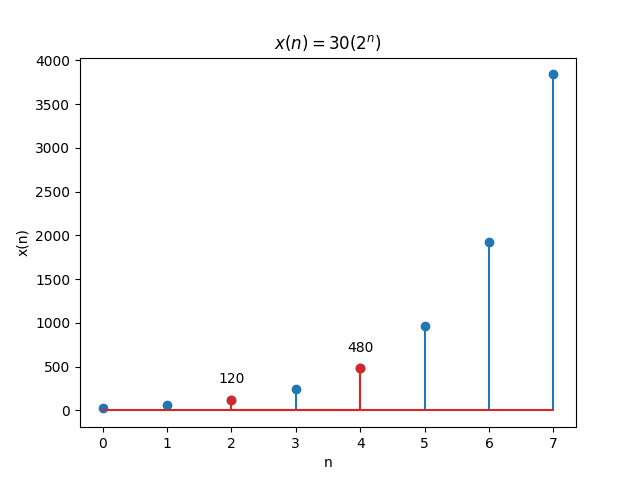
\includegraphics[width=\columnwidth]{figs/11_9_3_30.png}
    \caption{Plot of $x(n)$ vs $n$. See \tabref{tab:1} for details.}
    \label{fig:1}
\end{figure}
Let Z-transform of $x(n)$ be $X(z)$.
\begin{align}
X(z) &= \sum_{n = -\infty}^{\infty} x(n)u(n)z^{-n} \\
X(z) &= \sum_{n = 0}^{\infty} x(0)(r^n)(z^{-n}) \\
X(z) &= x(0)\lim_{n\to\infty}\sum_{i = 0}^{n}(\frac{r}{z})^i
\end{align}
\begin{enumerate}
\item If $|z| > r$:
\begin{align}
X(z) &= \frac{30}{1 - \frac{2}{z}} \\
X(z) &= \frac{30z}{z - 2}
\end{align}
\item If $|z| \le r$:
\begin{align}
X(z) \to \infty
\end{align}
\end{enumerate}
\begin{align}
\implies X(z) = \frac{30z}{z - 2} \quad |z| > 2
\end{align}
\end{document}